% Options for packages loaded elsewhere
\PassOptionsToPackage{unicode}{hyperref}
\PassOptionsToPackage{hyphens}{url}
\PassOptionsToPackage{dvipsnames,svgnames,x11names}{xcolor}
\documentclass[
  brazilian,
  12pt,
  a4paper,
]{article}
\usepackage{xcolor}
\usepackage[left=2cm, top=2cm, bottom=2cm, right=2cm]{geometry}
\usepackage{amsmath,amssymb}
\setcounter{secnumdepth}{5}
\usepackage{iftex}
\ifPDFTeX
  \usepackage[T1]{fontenc}
  \usepackage[utf8]{inputenc}
  \usepackage{textcomp} % provide euro and other symbols
\else % if luatex or xetex
  \usepackage{unicode-math} % this also loads fontspec
  \defaultfontfeatures{Scale=MatchLowercase}
  \defaultfontfeatures[\rmfamily]{Ligatures=TeX,Scale=1}
\fi
\usepackage{lmodern}
\ifPDFTeX\else
  % xetex/luatex font selection
\fi
% Use upquote if available, for straight quotes in verbatim environments
\IfFileExists{upquote.sty}{\usepackage{upquote}}{}
\IfFileExists{microtype.sty}{% use microtype if available
  \usepackage[]{microtype}
  \UseMicrotypeSet[protrusion]{basicmath} % disable protrusion for tt fonts
}{}
\usepackage{setspace}
\makeatletter
\@ifundefined{KOMAClassName}{% if non-KOMA class
  \IfFileExists{parskip.sty}{%
    \usepackage{parskip}
  }{% else
    \setlength{\parindent}{0pt}
    \setlength{\parskip}{6pt plus 2pt minus 1pt}}
}{% if KOMA class
  \KOMAoptions{parskip=half}}
\makeatother
\usepackage{color}
\usepackage{fancyvrb}
\newcommand{\VerbBar}{|}
\newcommand{\VERB}{\Verb[commandchars=\\\{\}]}
\DefineVerbatimEnvironment{Highlighting}{Verbatim}{commandchars=\\\{\}}
% Add ',fontsize=\small' for more characters per line
\usepackage{framed}
\definecolor{shadecolor}{RGB}{241,243,245}
\newenvironment{Shaded}{\begin{snugshade}}{\end{snugshade}}
\newcommand{\AlertTok}[1]{\textcolor[rgb]{0.68,0.00,0.00}{#1}}
\newcommand{\AnnotationTok}[1]{\textcolor[rgb]{0.37,0.37,0.37}{#1}}
\newcommand{\AttributeTok}[1]{\textcolor[rgb]{0.40,0.45,0.13}{#1}}
\newcommand{\BaseNTok}[1]{\textcolor[rgb]{0.68,0.00,0.00}{#1}}
\newcommand{\BuiltInTok}[1]{\textcolor[rgb]{0.00,0.46,0.62}{#1}}
\newcommand{\CharTok}[1]{\textcolor[rgb]{0.13,0.47,0.30}{#1}}
\newcommand{\CommentTok}[1]{\textcolor[rgb]{0.37,0.37,0.37}{#1}}
\newcommand{\CommentVarTok}[1]{\textcolor[rgb]{0.37,0.37,0.37}{\textit{#1}}}
\newcommand{\ConstantTok}[1]{\textcolor[rgb]{0.56,0.35,0.01}{#1}}
\newcommand{\ControlFlowTok}[1]{\textcolor[rgb]{0.00,0.46,0.62}{#1}}
\newcommand{\DataTypeTok}[1]{\textcolor[rgb]{0.68,0.00,0.00}{#1}}
\newcommand{\DecValTok}[1]{\textcolor[rgb]{0.68,0.00,0.00}{#1}}
\newcommand{\DocumentationTok}[1]{\textcolor[rgb]{0.37,0.37,0.37}{\textit{#1}}}
\newcommand{\ErrorTok}[1]{\textcolor[rgb]{0.68,0.00,0.00}{#1}}
\newcommand{\ExtensionTok}[1]{\textcolor[rgb]{0.00,0.46,0.62}{#1}}
\newcommand{\FloatTok}[1]{\textcolor[rgb]{0.68,0.00,0.00}{#1}}
\newcommand{\FunctionTok}[1]{\textcolor[rgb]{0.28,0.35,0.67}{#1}}
\newcommand{\ImportTok}[1]{\textcolor[rgb]{0.00,0.46,0.62}{#1}}
\newcommand{\InformationTok}[1]{\textcolor[rgb]{0.37,0.37,0.37}{#1}}
\newcommand{\KeywordTok}[1]{\textcolor[rgb]{0.00,0.46,0.62}{#1}}
\newcommand{\NormalTok}[1]{\textcolor[rgb]{0.00,0.46,0.62}{#1}}
\newcommand{\OperatorTok}[1]{\textcolor[rgb]{0.37,0.37,0.37}{#1}}
\newcommand{\OtherTok}[1]{\textcolor[rgb]{0.00,0.46,0.62}{#1}}
\newcommand{\PreprocessorTok}[1]{\textcolor[rgb]{0.68,0.00,0.00}{#1}}
\newcommand{\RegionMarkerTok}[1]{\textcolor[rgb]{0.00,0.46,0.62}{#1}}
\newcommand{\SpecialCharTok}[1]{\textcolor[rgb]{0.37,0.37,0.37}{#1}}
\newcommand{\SpecialStringTok}[1]{\textcolor[rgb]{0.13,0.47,0.30}{#1}}
\newcommand{\StringTok}[1]{\textcolor[rgb]{0.13,0.47,0.30}{#1}}
\newcommand{\VariableTok}[1]{\textcolor[rgb]{0.07,0.07,0.07}{#1}}
\newcommand{\VerbatimStringTok}[1]{\textcolor[rgb]{0.13,0.47,0.30}{#1}}
\newcommand{\WarningTok}[1]{\textcolor[rgb]{0.37,0.37,0.37}{\textit{#1}}}
\usepackage{longtable,booktabs,array}
\usepackage{calc} % for calculating minipage widths
% Correct order of tables after \paragraph or \subparagraph
\usepackage{etoolbox}
\makeatletter
\patchcmd\longtable{\par}{\if@noskipsec\mbox{}\fi\par}{}{}
\makeatother
% Allow footnotes in longtable head/foot
\IfFileExists{footnotehyper.sty}{\usepackage{footnotehyper}}{\usepackage{footnote}}
\makesavenoteenv{longtable}
\usepackage{graphicx}
\makeatletter
\newsavebox\pandoc@box
\newcommand*\pandocbounded[1]{% scales image to fit in text height/width
  \sbox\pandoc@box{#1}%
  \Gscale@div\@tempa{\textheight}{\dimexpr\ht\pandoc@box+\dp\pandoc@box\relax}%
  \Gscale@div\@tempb{\linewidth}{\wd\pandoc@box}%
  \ifdim\@tempb\p@<\@tempa\p@\let\@tempa\@tempb\fi% select the smaller of both
  \ifdim\@tempa\p@<\p@\scalebox{\@tempa}{\usebox\pandoc@box}%
  \else\usebox{\pandoc@box}%
  \fi%
}
% Set default figure placement to htbp
\def\fps@figure{htbp}
\makeatother
\ifLuaTeX
\usepackage[bidi=basic]{babel}
\else
\usepackage[bidi=default]{babel}
\fi
% get rid of language-specific shorthands (see #6817):
\let\LanguageShortHands\languageshorthands
\def\languageshorthands#1{}
\setlength{\emergencystretch}{3em} % prevent overfull lines
\providecommand{\tightlist}{%
  \setlength{\itemsep}{0pt}\setlength{\parskip}{0pt}}
\usepackage{setspace}
\setcounter{page}{-0}
\setlength{\parindent}{1.25cm}
\usepackage{cancel}
\usepackage{booktabs}
\usepackage{amsmath}
\usepackage{xcolor}
\renewcommand{\CancelColor}{\color{red}}
\usepackage[most]{tcolorbox}
\usepackage{slashbox}
\usepackage{pict2e}
\usepackage{enumitem}
\usepackage{graphicx}
\usepackage{bookmark}
\IfFileExists{xurl.sty}{\usepackage{xurl}}{} % add URL line breaks if available
\urlstyle{same}
\hypersetup{
  pdflang={pt-br},
  colorlinks=true,
  linkcolor={black},
  filecolor={Maroon},
  citecolor={Blue},
  urlcolor={Blue},
  pdfcreator={LaTeX via pandoc}}

\author{}
\date{\vspace{-2.5em}}

\begin{document}

\setstretch{1.5}
\thispagestyle{empty}

\begin{center}
\fontsize{12pt}{14pt}\selectfont
\singlespacing
  UNIVERSIDADE ESTADUAL DE MARINGÁ\\
  PROGRAMA DE PÓS-GRADUAÇÃO EM ENGENHARIA DE ALIMENTOS - PEG\\
  ESTATÍSTICA APLICADA - Prof. Dra. Emília\\
\end{center}

\begin{flushleft}
\fontsize{12pt}{14pt}\selectfont
\singlespacing
    \textbf{Acadêmico:} Jessica Hemily de Sá Gonçalves \\
    \textbf{Artigo}: Feeding with plant powders increases longevity and body weight of Western honeybee workers (Apis mellifera)
  \end{flushleft}

\fontsize{9pt}{11pt}\selectfont

\begin{itemize}
\tightlist
\item
  Artigo disponível em:
  \url{https://link.springer.com/article/10.1007/s13592-024-01094-4}
\end{itemize}

\section{Objetivo do estudo}\label{objetivo-do-estudo}

Este trabalho reproduz as principais análises estatísticas do artigo
\emph{Feeding with plant powders increases longevity and body weight of
Western honeybee workers (Apis mellifera)} (Brown et al., 2024). O
estudo investigou se a suplementação alimentar de abelhas-operárias
(\emph{Apis mellifera}) com diferentes pós vegetais poderia melhorar
indicadores de saúde das colônias.

Para isso, os autores compararam um grupo controle alimentado apenas com
solução de sacarose a 50\% com 12 grupos experimentais que receberam a
mesma solução enriquecida com diferentes pós vegetais. Foram avaliados
três desfechos principais:

\begin{itemize}
\tightlist
\item
  \textbf{Consumo de sacarose}, para verificar se os diferentes
  suplementos alteravam o padrão de alimentação das abelhas;
\item
  \textbf{Peso seco corporal}, utilizado como indicador do estado
  nutricional e da condição física dos indivíduos;
\item
  \textbf{Longevidade (sobrevivência)}, utilizada para avaliar o efeito
  dos suplementos sobre o tempo de vida das abelhas.
\end{itemize}

Ao longo deste documento, cada uma dessas variáveis será analisada
utilizando a mesma metodologia estatística descrita no artigo,
reproduzindo os modelos, testes e gráficos apresentados pelos autores.

\section{Bibliotecas}\label{bibliotecas}

\begin{Shaded}
\begin{Highlighting}[]
\FunctionTok{library}\NormalTok{(readxl)}
\FunctionTok{library}\NormalTok{(dplyr)}
\FunctionTok{library}\NormalTok{(psych)}
\FunctionTok{library}\NormalTok{(FSA)}
\FunctionTok{library}\NormalTok{(lme4)}
\FunctionTok{library}\NormalTok{(lmerTest)}
\FunctionTok{library}\NormalTok{(nlme)}
\FunctionTok{library}\NormalTok{(car)}
\FunctionTok{library}\NormalTok{(fitdistrplus)}
\FunctionTok{library}\NormalTok{(gtools)}
\FunctionTok{library}\NormalTok{(ggplot2)}
\FunctionTok{library}\NormalTok{(moments)}
\FunctionTok{library}\NormalTok{(knitr)}
\end{Highlighting}
\end{Shaded}

\section{Estratégia estatística}\label{estratuxe9gia-estatuxedstica}

As análises estatísticas foram divididas em três etapas, cada uma
destinada à avaliação de uma variável resposta.

\subsection{Consumo de sacarose}\label{consumo-de-sacarose}

\begin{itemize}
\item
  \textbf{Variável resposta:} Consumo diário de sacarose (loss).
\item
  \textbf{Variáveis explicativas:} Tratamento (Treatment) e tempo (day).
\item
  \textbf{Modelo empregado:} Regressão linear com efeito polinomial de
  terceiro grau.
\end{itemize}

\[
\text{loss}=\beta_0+\beta_1\text{Treatment}+\beta_2\text{day}
+\beta_3\text{day}^2+\beta_4\text{day}^3+\varepsilon
\]

Posteriormente, foram realizadas comparações múltiplas entre cada
tratamento e o grupo controle utilizando o teste de Dunnett.

\subsection{Peso seco corporal}\label{peso-seco-corporal}

\begin{itemize}
\item
  \textbf{Variável resposta:} Peso seco corporal (dry\_weight).
\item
  \textbf{Variável explicativa:} Tempo (day).
\end{itemize}

Inicialmente foi ajustado o modelo

\[
\text{dry\_weight}=\beta_0 + \beta_1*\text{day} + \varepsilon
\]

Como os resíduos não apresentaram distribuição normal, foram utilizados
o teste de Kruskal-Wallis e comparações múltiplas pelo teste de Wilcoxon
com correção de Benjamini-Hochberg.

\subsection{Longevidade}\label{longevidade}

\begin{itemize}
\tightlist
\item
  \textbf{Variável resposta:} Tempo até a morte (day).
\item
  \textbf{Variável explicativa:} Tratamento (Treatment).
\end{itemize}

A função de sobrevivência foi estimada pelo estimador de Kaplan-Meier,

\[
\hat{S}(t)=\prod_{t_i\le t}\left(1-\frac{d_i}{n_i}\right)
\]

e as curvas foram comparadas por meio do teste Log-rank, com correção de
Benjamini-Hochberg para comparações múltiplas.

\section{Análise do Consumo de
Sacarose}\label{anuxe1lise-do-consumo-de-sacarose}

\subsection{Delineamento do experimento}

O experimento foi conduzido utilizando um total de 2028 abelhas
operárias (\textit{Apis mellifera}), distribuídas em 13 tratamentos.
Cada tratamento foi composto por seis gaiolas (réplicas), contendo 26
abelhas em cada uma, totalizando

\[
13 \times 6 \times 26 = 2028 \text{ abelhas}.
\]

Os tratamentos consistiram em uma solução de sacarose a 50\%
(\textit{controle}) ou em solução de sacarose acrescida de um dos 12
diferentes pós vegetais avaliados.

\textbf{Unidade experimental:} Gaiola - 78 gaiolas avaliadas por até 69
dias.

\subsection{Consumo de sacarose}

O consumo de sacarose foi avaliado diariamente durante todo o período
experimental. Para isso, as seringas contendo a solução alimentar foram
pesadas a cada 24 horas. A diferença entre duas pesagens consecutivas
representou a quantidade de alimento consumida pelas abelhas durante
aquele intervalo de tempo.

Em seguida, esse valor foi dividido pelo número de abelhas vivas
presentes em cada gaiola, obtendo-se o consumo médio diário de sacarose
por abelha.

\subsection{Objetivo da análise}

A análise do consumo de sacarose teve como objetivo verificar se a
adição de diferentes pós vegetais à solução de sacarose influenciava o
consumo alimentar das abelhas, isto é, se algum tratamento levava a um
aumento ou redução na ingestão da solução.

Os resultados mostraram que, de maneira geral, não houve diferenças
significativas no consumo de sacarose entre os tratamentos, indicando
que a adição dos pós vegetais não alterou o comportamento alimentar das
abelhas.

\subsection{Carregamento e Preparação dos
Dados}\label{carregamento-e-preparauxe7uxe3o-dos-dados}

\begin{longtable}[]{@{}rlrr@{}}
\caption{Primeiras observações da base de dados de consumo de
sacarose.}\tabularnewline
\toprule\noalign{}
cage & Treatment & day & loss \\
\midrule\noalign{}
\endfirsthead
\toprule\noalign{}
cage & Treatment & day & loss \\
\midrule\noalign{}
\endhead
\bottomrule\noalign{}
\endlastfoot
67 & Urtica dioica & 7 & 62.36 \\
12 & Calendulae officinalis & 8 & 62.36 \\
55 & Curcuma longa & 17 & 62.21 \\
83 & Chlorella vulgaris & 14 & 62.21 \\
93 & Hypericum spp & 8 & 62.18 \\
56 & Curcuma longa & 16 & 62.18 \\
76 & Rosa canina & 16 & 62.02 \\
\end{longtable}

\begin{longtable}[]{@{}rlrr@{}}
\toprule\noalign{}
cage & Treatment & day & loss \\
\midrule\noalign{}
\endhead
\bottomrule\noalign{}
\endlastfoot
122 & Moringa oleifera & 14 & 61.863 \\
27 & Melissa officinalis & 62 & 61.811 \\
33 & Quercus spp & 68 & 61.762 \\
122 & Moringa oleifera & 39 & 61.733 \\
37 & Quercus spp & 14 & 61.600 \\
95 & Hypericum spp & 8 & 61.572 \\
25 & Melissa officinalis & 14 & 61.545 \\
127 & Moringa oleifera & 6 & 61.449 \\
115 & Trigonella foenum-graecum & 7 & 61.424 \\
\end{longtable}

\begin{itemize}
\tightlist
\item
  \textbf{Variável resposta:} Consumo diário de sacarose (loss).
\end{itemize}

\pandocbounded{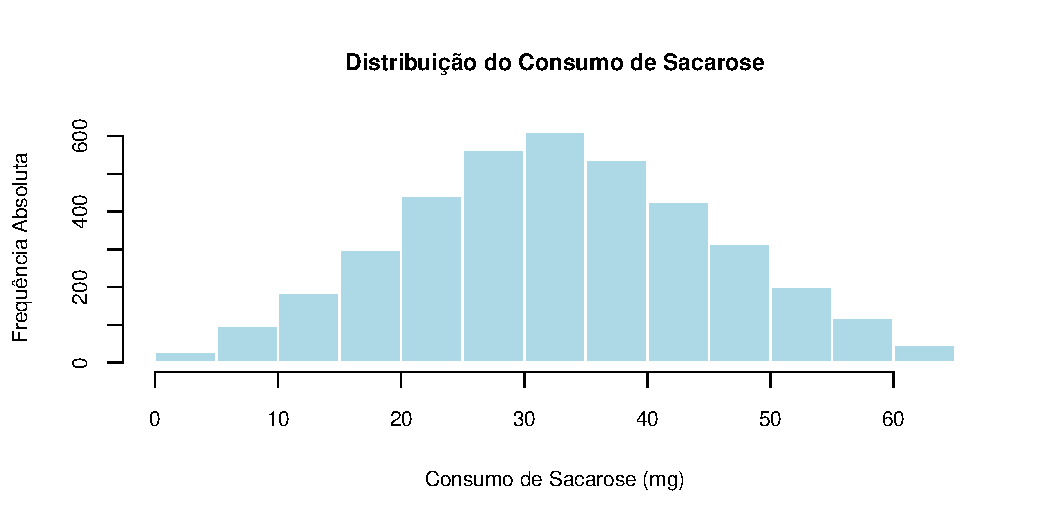
\includegraphics[keepaspectratio]{codigo_abelhas_files/figure-latex/unnamed-chunk-4-1.pdf}}

\begin{itemize}
\tightlist
\item
  \textbf{Variáveis explicativas:} Tratamento (Treatment) e tempo (day).
\end{itemize}

\pandocbounded{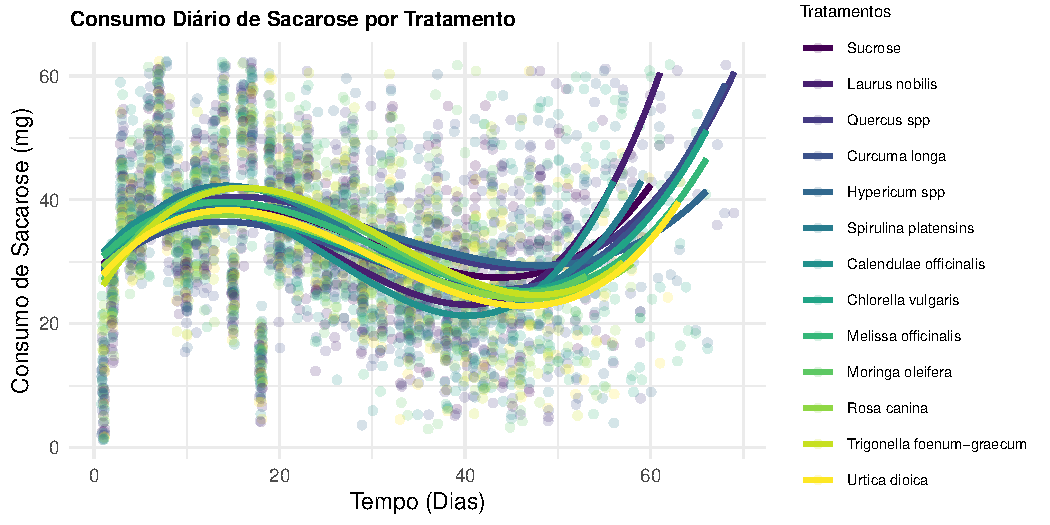
\includegraphics[keepaspectratio]{codigo_abelhas_files/figure-latex/unnamed-chunk-5-1.pdf}}

\subsection{Ajuste do Modelo Polinomial (Regressão
Cúbica)}\label{ajuste-do-modelo-polinomial-regressuxe3o-cuxfabica}

Como o consumo de sacarose ao longo dos dias não segue uma linha reta
simples, ajustamos um modelo linear com polinômio de 3º grau (poly(day,
3, raw=T)) para a variável temporal. Isso permite capturar curvas em
formato de ``S'' no consumo de alimentos. O argumento raw=TRUE é
utilizado para gerar polinômios brutos (\(x, x^2, x^3\)), facilitando a
interpretação matemática direta da equação do modelo.

\[
\text{loss}=\beta_0+\beta_1\text{Treatment}+\beta_2\text{day}
+\beta_3\text{day}^2+\beta_4\text{day}^3+\varepsilon
\]

\begin{Shaded}
\begin{Highlighting}[]
\NormalTok{df\_loss}\SpecialCharTok{$}\NormalTok{Treatment }\OtherTok{\textless{}{-}} \FunctionTok{as.factor}\NormalTok{(df\_loss}\SpecialCharTok{$}\NormalTok{Treatment)}
\NormalTok{df\_loss}\SpecialCharTok{$}\NormalTok{Treatment }\OtherTok{\textless{}{-}} \FunctionTok{ordered}\NormalTok{(df\_loss}\SpecialCharTok{$}\NormalTok{Treatment,}
                     \AttributeTok{levels =} \FunctionTok{c}\NormalTok{(}\StringTok{"Sucrose"}\NormalTok{,}\StringTok{"Laurus nobilis"}\NormalTok{,}\StringTok{"Quercus spp"}\NormalTok{, }\StringTok{"Curcuma longa"}\NormalTok{,}
                                \StringTok{"Hypericum spp"}\NormalTok{,}\StringTok{"Spirulina platensins"}\NormalTok{, }\StringTok{"Calendulae officinalis"}\NormalTok{,}
                                \StringTok{"Chlorella vulgaris"}\NormalTok{, }\StringTok{"Melissa officinalis"}\NormalTok{,}\StringTok{"Moringa oleifera"}\NormalTok{,}
                                \StringTok{"Rosa canina"}\NormalTok{,}\StringTok{"Trigonella foenum{-}graecum"}\NormalTok{, }\StringTok{"Urtica dioica"}\NormalTok{))}
\FunctionTok{levels}\NormalTok{(df\_loss}\SpecialCharTok{$}\NormalTok{Treatment)}
\end{Highlighting}
\end{Shaded}

\begin{verbatim}
##  [1] "Sucrose"                   "Laurus nobilis"           
##  [3] "Quercus spp"               "Curcuma longa"            
##  [5] "Hypericum spp"             "Spirulina platensins"     
##  [7] "Calendulae officinalis"    "Chlorella vulgaris"       
##  [9] "Melissa officinalis"       "Moringa oleifera"         
## [11] "Rosa canina"               "Trigonella foenum-graecum"
## [13] "Urtica dioica"
\end{verbatim}

\begin{Shaded}
\begin{Highlighting}[]
\NormalTok{best }\OtherTok{=} \FunctionTok{lm}\NormalTok{(loss }\SpecialCharTok{\textasciitilde{}} \FunctionTok{factor}\NormalTok{(Treatment) }\SpecialCharTok{+} \FunctionTok{poly}\NormalTok{(day,}\DecValTok{3}\NormalTok{, }\AttributeTok{raw=}\NormalTok{T), }\AttributeTok{data=}\NormalTok{df\_loss)}
\FunctionTok{summary}\NormalTok{(best)}
\end{Highlighting}
\end{Shaded}

\begin{verbatim}
## 
## Call:
## lm(formula = loss ~ factor(Treatment) + poly(day, 3, raw = T), 
##     data = df_loss)
## 
## Residuals:
##     Min      1Q  Median      3Q     Max 
## -36.475  -7.390  -0.220   7.497  36.786 
## 
## Coefficients:
##                          Estimate Std. Error t value Pr(>|t|)    
## (Intercept)             2.798e+01  7.126e-01  39.267  < 2e-16 ***
## factor(Treatment).L    -7.319e-01  6.657e-01  -1.099  0.27166    
## factor(Treatment).Q    -3.447e-01  6.663e-01  -0.517  0.60497    
## factor(Treatment).C    -3.283e-01  6.640e-01  -0.494  0.62106    
## factor(Treatment)^4    -9.200e-01  6.654e-01  -1.383  0.16687    
## factor(Treatment)^5    -1.740e+00  6.586e-01  -2.642  0.00829 ** 
## factor(Treatment)^6     1.003e+00  6.691e-01   1.499  0.13401    
## factor(Treatment)^7    -9.669e-01  6.609e-01  -1.463  0.14354    
## factor(Treatment)^8    -7.652e-01  6.557e-01  -1.167  0.24333    
## factor(Treatment)^9    -3.650e+00  6.621e-01  -5.512 3.77e-08 ***
## factor(Treatment)^10    1.751e+00  6.697e-01   2.615  0.00896 ** 
## factor(Treatment)^11   -1.430e+00  6.501e-01  -2.199  0.02794 *  
## factor(Treatment)^12   -6.241e-01  6.604e-01  -0.945  0.34473    
## poly(day, 3, raw = T)1  1.745e+00  1.006e-01  17.350  < 2e-16 ***
## poly(day, 3, raw = T)2 -8.067e-02  3.851e-03 -20.950  < 2e-16 ***
## poly(day, 3, raw = T)3  9.029e-04  4.214e-05  21.427  < 2e-16 ***
## ---
## Signif. codes:  0 '***' 0.001 '**' 0.01 '*' 0.05 '.' 0.1 ' ' 1
## 
## Residual standard error: 11.38 on 3852 degrees of freedom
## Multiple R-squared:  0.169,  Adjusted R-squared:  0.1658 
## F-statistic: 52.23 on 15 and 3852 DF,  p-value: < 2.2e-16
\end{verbatim}

\subsection{Análise de Variância para Significância da Regressão em
Regressão
Múltipla}\label{anuxe1lise-de-variuxe2ncia-para-significuxe2ncia-da-regressuxe3o-em-regressuxe3o-muxfaltipla}

Para verificar a significância global do modelo de regressão múltipla
ajustado para o consumo de sacarose, realizamos o teste \(F\) da Análise
de Variância (ANOVA). Esse teste avalia simultaneamente se algum dos
coeficientes associados aos tratamentos ou aos termos polinomiais do
tempo (\(day\), \(day^2\) e \(day^3\)) é estatisticamente diferente de
zero.

As hipóteses testadas são estruturadas da seguinte forma:

\begin{itemize}
    \item \textbf{Hipótese Nula ($H_0$):} $\beta_1 = \beta_2 = \beta_3 = \beta_4 = 0$
    
    A hipótese nula assume que nenhum dos tratamentos com pós vegetais e nenhuma das potências do tempo possuem efeito sobre o consumo de sacarose. O modelo prediz tão bem quanto a média amostral ($\bar{Y}$).
    
    \item \textbf{Hipótese Alternativa ($H_1$):} Pelo menos um $\beta_j \neq 0$ (para $j = 1, 2, 3, 4$).
    
    A hipótese alternativa afirma que pelo menos uma das variáveis explicativas (seja um tratamento específico ou o comportamento temporal do componente polinomial) possui efeito significativo para explicar a variação no consumo de sacarose das abelhas.
\end{itemize}

Se o p-valor associado à estatística \(F\) do teste for menor que o
nível de significância adotado (\(\alpha = 0,05\)), rejeita-se \(H_0\),
justificando a relevância do modelo múltiplo completo adotado pelos
autores.

\begin{figure}
    \centering
    \includegraphics[width=0.8\linewidth]{anova_tabela.png}
\caption{Tabela de análise de variância (ANOVA) para modelos de regressão linear. Fonte: Introduction to Linear Regression Analysis, Montgomery et al. (2021, p. 85).}
    \label{fig:esquema_projeto}
\end{figure}

\subsubsection{SQ regressão}\label{sq-regressuxe3o}

A Soma de Quadrados da Regressão (SQReg) quantifica a variabilidade
explicada pelo modelo ajustado e é dada por

\[
SQ_{\text{Reg}}
=
\sum_{i=1}^{n}(\hat{y}_i-\bar{y})^2,
\]

em que \(\hat{y}_i\) corresponde ao valor ajustado (predito) pelo modelo
para a \(i\)-ésima observação.

\begin{Shaded}
\begin{Highlighting}[]
\NormalTok{media }\OtherTok{\textless{}{-}} \FunctionTok{mean}\NormalTok{(df\_loss}\SpecialCharTok{$}\NormalTok{loss)}
\NormalTok{yi }\OtherTok{\textless{}{-}}\NormalTok{ best}\SpecialCharTok{$}\NormalTok{fitted.values}
\NormalTok{SQ\_reg }\OtherTok{\textless{}{-}} \FunctionTok{sum}\NormalTok{((yi }\SpecialCharTok{{-}}\NormalTok{ media)}\SpecialCharTok{\^{}}\DecValTok{2}\NormalTok{)}
\NormalTok{npar }\OtherTok{\textless{}{-}} \FunctionTok{length}\NormalTok{(best}\SpecialCharTok{$}\NormalTok{coefficients)   }\CommentTok{\# p}
\NormalTok{gl\_reg }\OtherTok{\textless{}{-}}\NormalTok{ npar }\SpecialCharTok{{-}} \DecValTok{1}
\FunctionTok{data.frame}\NormalTok{(}\StringTok{"SQ\_reg"}\OtherTok{=}\NormalTok{SQ\_reg, }\StringTok{"gl\_reg"} \OtherTok{=}\NormalTok{ gl\_reg)}
\end{Highlighting}
\end{Shaded}

\begin{longtable}[]{@{}rr@{}}
\toprule\noalign{}
SQ\_reg & gl\_reg \\
\midrule\noalign{}
\endhead
\bottomrule\noalign{}
\endlastfoot
101442.8 & 15 \\
\end{longtable}

\subsubsection{SQ resíduo}\label{sq-resuxedduo}

A Soma de Quadrados dos Resíduos (SQRes) representa a variabilidade não
explicada pelo modelo e é calculada por

\[
SQ_{\text{Res}}
=
\sum_{i=1}^{n}(y_i-\hat{y}_i)^2.
\]

\begin{Shaded}
\begin{Highlighting}[]
\NormalTok{media }\OtherTok{\textless{}{-}} \FunctionTok{mean}\NormalTok{(df\_loss}\SpecialCharTok{$}\NormalTok{loss)}
\NormalTok{SQ\_res }\OtherTok{\textless{}{-}} \FunctionTok{sum}\NormalTok{((df\_loss}\SpecialCharTok{$}\NormalTok{loss }\SpecialCharTok{{-}}\NormalTok{ yi)}\SpecialCharTok{\^{}}\DecValTok{2}\NormalTok{)}
\NormalTok{npar }\OtherTok{\textless{}{-}} \FunctionTok{length}\NormalTok{(best}\SpecialCharTok{$}\NormalTok{coefficients)   }\CommentTok{\#p}
\NormalTok{n }\OtherTok{\textless{}{-}} \FunctionTok{length}\NormalTok{(best}\SpecialCharTok{$}\NormalTok{fitted.values)}
\NormalTok{gl\_res }\OtherTok{\textless{}{-}}\NormalTok{ n}\SpecialCharTok{{-}}\NormalTok{npar  }\CommentTok{\# n {-} p}
\FunctionTok{data.frame}\NormalTok{(}\StringTok{"SQ\_res"}\OtherTok{=}\NormalTok{SQ\_res, }\StringTok{"gl\_res"} \OtherTok{=}\NormalTok{ gl\_res)}
\end{Highlighting}
\end{Shaded}

\begin{longtable}[]{@{}rr@{}}
\toprule\noalign{}
SQ\_res & gl\_res \\
\midrule\noalign{}
\endhead
\bottomrule\noalign{}
\endlastfoot
498777.3 & 3852 \\
\end{longtable}

\subsubsection{SQ total}\label{sq-total}

A Soma de Quadrados Total (SQT) mede a variabilidade total da variável
resposta em torno de sua média e é calculada por:

\[
SQ_{\text{Total}}
=
\sum_{i=1}^{n}(y_i-\bar{y})^2,
\]

em que \(y_i\) representa o valor observado da variável resposta,
\(\bar{y}\) é a média amostral da variável resposta e \(n\) é o número
de observações.

\begin{Shaded}
\begin{Highlighting}[]
\NormalTok{media }\OtherTok{\textless{}{-}} \FunctionTok{mean}\NormalTok{(df\_loss}\SpecialCharTok{$}\NormalTok{loss)}
\NormalTok{SQ\_t }\OtherTok{\textless{}{-}} \FunctionTok{sum}\NormalTok{((df\_loss}\SpecialCharTok{$}\NormalTok{loss }\SpecialCharTok{{-}}\NormalTok{ media)}\SpecialCharTok{\^{}}\DecValTok{2}\NormalTok{)}
\NormalTok{gl\_t }\OtherTok{\textless{}{-}} \FunctionTok{length}\NormalTok{(best}\SpecialCharTok{$}\NormalTok{fitted.values)}\SpecialCharTok{{-}} \DecValTok{1}
\FunctionTok{data.frame}\NormalTok{(}\StringTok{"SQ\_T"}\OtherTok{=}\NormalTok{SQ\_t, }\StringTok{"gl\_t"} \OtherTok{=}\NormalTok{ gl\_t)}
\end{Highlighting}
\end{Shaded}

\begin{longtable}[]{@{}rr@{}}
\toprule\noalign{}
SQ\_T & gl\_t \\
\midrule\noalign{}
\endhead
\bottomrule\noalign{}
\endlastfoot
600220.1 & 3867 \\
\end{longtable}

Uma propriedade fundamental da regressão linear é a decomposição da
variabilidade total, dada por

\[
SQ_{\text{Total}}
=
SQ_{\text{Reg}}
+
SQ_{\text{Res}}.
\]

\begin{Shaded}
\begin{Highlighting}[]
\NormalTok{total }\OtherTok{\textless{}{-}}\NormalTok{ SQ\_reg }\SpecialCharTok{+}\NormalTok{ SQ\_res}
\NormalTok{total}
\end{Highlighting}
\end{Shaded}

\begin{verbatim}
## [1] 600220.1
\end{verbatim}

\subsubsection{TABELA ANOVA}\label{tabela-anova}

\begin{Shaded}
\begin{Highlighting}[]
\NormalTok{QM\_reg }\OtherTok{\textless{}{-}}\NormalTok{ SQ\_reg }\SpecialCharTok{/}\NormalTok{ gl\_reg}
\NormalTok{QM\_res }\OtherTok{\textless{}{-}}\NormalTok{ SQ\_res }\SpecialCharTok{/}\NormalTok{ gl\_res}
\NormalTok{F\_reg }\OtherTok{\textless{}{-}}\NormalTok{ QM\_reg }\SpecialCharTok{/}\NormalTok{ QM\_res}
\NormalTok{tab\_anova }\OtherTok{\textless{}{-}} \FunctionTok{data.frame}\NormalTok{(}\AttributeTok{Fonte =} \FunctionTok{c}\NormalTok{(}\StringTok{"Regressão"}\NormalTok{, }\StringTok{"Resíduo"}\NormalTok{, }\StringTok{"Total"}\NormalTok{),}
                        \AttributeTok{GL =} \FunctionTok{c}\NormalTok{(gl\_reg, gl\_res, gl\_t),}
                        \AttributeTok{SQ =} \FunctionTok{c}\NormalTok{(SQ\_reg, SQ\_res, SQ\_t),}
                        \AttributeTok{QM =} \FunctionTok{c}\NormalTok{(QM\_reg, QM\_res, }\ConstantTok{NA}\NormalTok{),}
                        \AttributeTok{F =} \FunctionTok{c}\NormalTok{(F\_reg, }\ConstantTok{NA}\NormalTok{, }\ConstantTok{NA}\NormalTok{))}
\NormalTok{tab\_anova}
\end{Highlighting}
\end{Shaded}

\begin{longtable}[]{@{}lrrrr@{}}
\toprule\noalign{}
Fonte & GL & SQ & QM & F \\
\midrule\noalign{}
\endhead
\bottomrule\noalign{}
\endlastfoot
Regressão & 15 & 101442.8 & 6762.8525 & 52.22873 \\
Resíduo & 3852 & 498777.3 & 129.4853 & NA \\
Total & 3867 & 600220.1 & NA & NA \\
\end{longtable}

A Tabela xx apresenta a análise de variância (ANOVA) do modelo de
regressão ajustado para o consumo de sacarose. A estatística de teste
utilizada é dada por

\[
F=\frac{\text{Quadrado Médio da Regressão }(QM_{\text{Reg}})}{\text{Quadrado Médio do Resíduo  }(QM_{\text{Res}})}=
\frac{\dfrac{SQ_{\text{Reg}}}{GL_{\text{Reg}}}}
{\dfrac{SQ_{\text{Res}}}{GL_{\text{Res}}}},
\]

em que:

\begin{itemize}
    \item \(SQ_{\text{Reg}}\): Soma de Quadrados da Regressão;
    \item \(SQ_{\text{Res}}\): Soma de Quadrados dos Resíduos;
    \item \(GL_{\text{Reg}}\): graus de liberdade da regressão;
    \item \(GL_{\text{Res}}\): graus de liberdade dos resíduos.
\end{itemize}

Essa estatística compara a variabilidade explicada pelo modelo com a
variabilidade residual. Valores de \(F\) próximos de 1 indicam que o
modelo não explica a variável resposta melhor do que o erro aleatório,
enquanto valores elevados sugerem que a variabilidade explicada é
substancialmente maior que a variabilidade residual.

No modelo ajustado, obteve-se \(F(15,3852)=52,23\), com
valor-\(p < 2,2\times10^{-16}\). O numerador possui 15 graus de
liberdade, correspondentes aos efeitos dos tratamentos e aos três termos
polinomiais do tempo, enquanto o denominador possui 3852 graus de
liberdade, associados aos resíduos do modelo.

\begin{itemize}  
\item O p-valor é calculado achando-se a área sob a curva de densidade após o ponto da estatística observada ($52,23$), formalizado por $P(F_{(15, 3852)} \ge 52,23)$. Como a distribuição $F$ decai de forma assintótica extremamente rápida, a probabilidade de se obter um valor tão alto quanto $52,23$ por puro acaso é infinitesimal. O valor exato ultrapassou a precisão matemática do sistema, resultando no teto estatístico aproximado de $p < 2,2 \times 10^{-16}$.
\end{itemize}

\begin{Shaded}
\begin{Highlighting}[]
\FunctionTok{qf}\NormalTok{(}\FloatTok{0.95}\NormalTok{,}\DecValTok{15}\NormalTok{,}\DecValTok{3852}\NormalTok{)}
\end{Highlighting}
\end{Shaded}

\begin{verbatim}
## [1] 1.668981
\end{verbatim}

Considerando o nível de significância de 5\%, rejeita-se a hipótese nula

\[
H_0:\beta_1=\beta_2=\cdots=\beta_{15}=0,
\]

que afirma que nenhum dos coeficientes associados às variáveis
explicativas difere de zero. Portanto, conclui-se que pelo menos um dos
efeitos incluídos no modelo contribui significativamente para explicar a
variação observada no consumo de sacarose.

Além disso, o coeficiente de determinação foi \(R^2=0,169\), indicando
que aproximadamente \(16,9\%\) da variabilidade do consumo de sacarose
foi explicada pelo conjunto das variáveis explicativas (tratamento e
tempo). O valor do coeficiente de determinação ajustado
(\(R^2_{aj}=0,166\)) foi muito próximo ao \(R^2\), sugerindo que a
inclusão dos termos no modelo foi adequada e não promoveu um aumento
artificial da capacidade explicativa.

O coeficiente de determinação (\(R^2\)) é definido por:

\[
R^2=\frac{SQ_{\text{Reg}}}{SQ_{\text{Total}}}
=1-\frac{SQ_{\text{Res}}}{SQ_{\text{Total}}},
\]

O coeficiente de determinação ajustado (\(R^2_{aj}\)) é dado por:

obs.: O \(R_{ajustado}^2\) pode aumentar ou diminuir, dependendo da
contribuição das covariáveis adicionadas. Diferentemente do \(R^2\) que
tem seu valor aumentado com a adição de covariáveis.

\[
R^2_{aj}
=
1-
\left(
\frac{SQ_{\text{Res}}/(n-p)}
{SQ_{\text{Total}}/(n-1)}
\right),
\]

\begin{Shaded}
\begin{Highlighting}[]
\NormalTok{r\_2 }\OtherTok{\textless{}{-}}\NormalTok{ SQ\_reg}\SpecialCharTok{/}\NormalTok{SQ\_t}
\NormalTok{r\_2ajustado }\OtherTok{\textless{}{-}} \DecValTok{1} \SpecialCharTok{{-}}\NormalTok{ (SQ\_res}\SpecialCharTok{/}\NormalTok{(n}\SpecialCharTok{{-}}\NormalTok{npar)) }\SpecialCharTok{/}\NormalTok{ (SQ\_t}\SpecialCharTok{/}\NormalTok{(n}\DecValTok{{-}1}\NormalTok{))}

\FunctionTok{data.frame}\NormalTok{(}\StringTok{"R quadrado"} \OtherTok{=} \FunctionTok{round}\NormalTok{(r\_2,}\DecValTok{3}\NormalTok{), }\StringTok{"R quadrado ajustado"} \OtherTok{=} \FunctionTok{round}\NormalTok{(r\_2ajustado,}\DecValTok{3}\NormalTok{))}
\end{Highlighting}
\end{Shaded}

\begin{longtable}[]{@{}rr@{}}
\toprule\noalign{}
R.quadrado & R.quadrado.ajustado \\
\midrule\noalign{}
\endhead
\bottomrule\noalign{}
\endlastfoot
0.169 & 0.166 \\
\end{longtable}

\newpage

\subsection{Diagnóstico do Modelo}\label{diagnuxf3stico-do-modelo}

O objetivo é checar os pressupostos de homocedasticidade (variância
constante) e a normalidade dos resíduos do modelo ajustado.

\begin{Shaded}
\begin{Highlighting}[]
\FunctionTok{par}\NormalTok{(}\AttributeTok{mfrow =} \FunctionTok{c}\NormalTok{(}\DecValTok{2}\NormalTok{,}\DecValTok{2}\NormalTok{))}
\FunctionTok{plot}\NormalTok{(best)}
\end{Highlighting}
\end{Shaded}

\pandocbounded{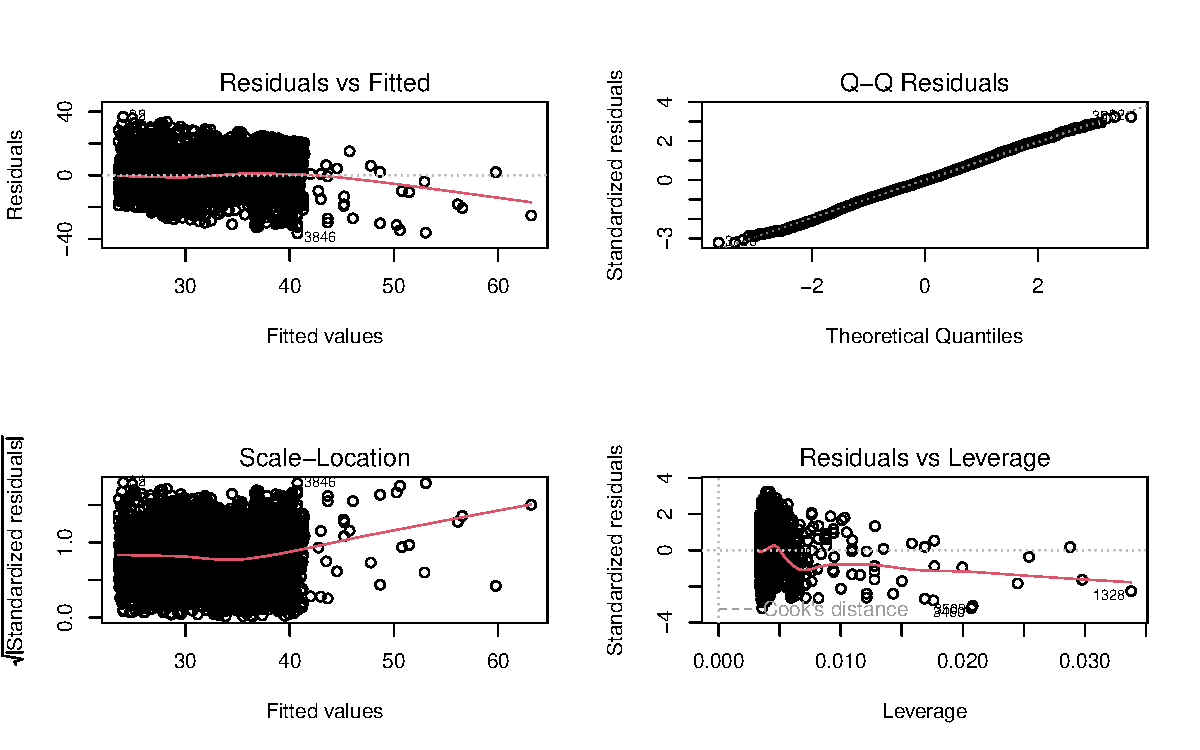
\includegraphics[keepaspectratio]{codigo_abelhas_files/figure-latex/unnamed-chunk-15-1.pdf}}

\begin{Shaded}
\begin{Highlighting}[]
\FunctionTok{par}\NormalTok{(}\AttributeTok{mfrow =} \FunctionTok{c}\NormalTok{(}\DecValTok{1}\NormalTok{,}\DecValTok{1}\NormalTok{))}
\FunctionTok{qqPlot}\NormalTok{(}\FunctionTok{residuals}\NormalTok{(best))}
\end{Highlighting}
\end{Shaded}

\pandocbounded{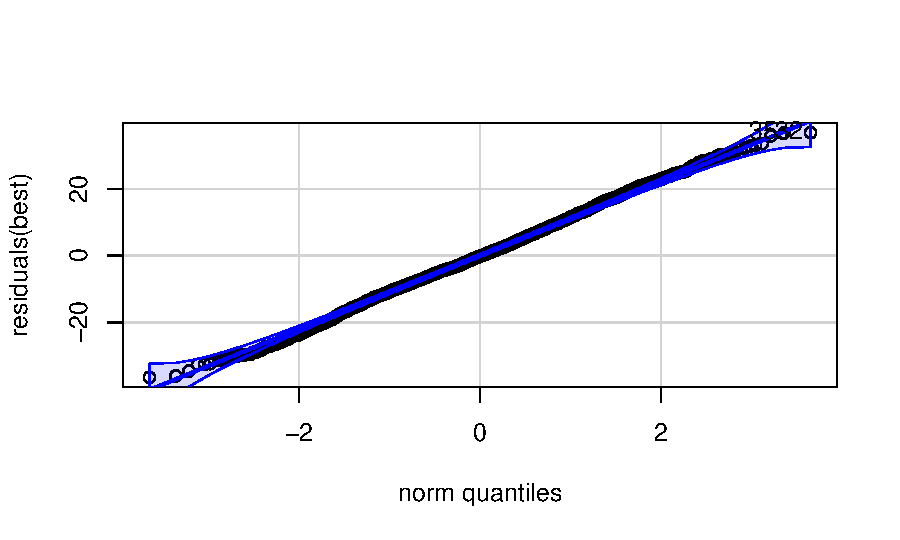
\includegraphics[keepaspectratio]{codigo_abelhas_files/figure-latex/unnamed-chunk-16-1.pdf}}

\begin{verbatim}
## [1] 32 35
\end{verbatim}

\section{Análise do Peso Seco Corporal (Dry Body
Weight)}\label{anuxe1lise-do-peso-seco-corporal-dry-body-weight}

O peso seco das abelhas foi utilizado como uma medida da biomassa
corporal, eliminando a influência da água presente no organismo. Para
isso, nos dias 7 e 14 do experimento, foram selecionadas aleatoriamente
três abelhas vivas de cada gaiola para pesagem.

Após a pesagem inicial, as abelhas foram congeladas e, ao término do
experimento, permaneceram em estufa de convecção a
\(65\,^{\circ}\mathrm{C}\) durante 96 horas. Em seguida, foram novamente
pesadas, sendo essa segunda medida denominada \textit{peso seco}.

Ao todo, foram obtidas \(13 \times 6 \times 2 \times 3 = 468\)
observações, correspondentes a:

\begin{itemize}
    \item 13 tratamentos;
    \item 6 gaiolas (réplicas) por tratamento;
    \item 2 momentos de avaliação (dias 7 e 14);
    \item 3 abelhas amostradas por gaiola em cada avaliação.
\end{itemize}

\subsection{Objetivo da análise}

A análise do peso seco teve como objetivo avaliar se a suplementação da
solução de sacarose com diferentes pós vegetais promovia aumento da
biomassa corporal das abelhas em comparação ao tratamento controle.

Os resultados indicaram que os tratamentos contendo
\textit{Quercus spp.}, \textit{Hypericum spp.},
\textit{Spirulina platensis}, \textit{Melissa officinalis},
\textit{Moringa oleifera} e \textit{Trigonella foenum-graecum}
proporcionaram aumento significativo no peso seco das abelhas em relação
ao grupo controle.

\subsection{Carregamento e Preparação dos
Dados}\label{carregamento-e-preparauxe7uxe3o-dos-dados-1}

\begin{Shaded}
\begin{Highlighting}[]
\NormalTok{df\_weight }\OtherTok{\textless{}{-}} \FunctionTok{read\_excel}\NormalTok{(}\StringTok{"Plant{-}Powder{-}All{-}Data{-}Final.xlsx"}\NormalTok{, }\AttributeTok{sheet =} \DecValTok{3}\NormalTok{)}
\NormalTok{df\_weight}\SpecialCharTok{$}\NormalTok{dry\_weight }\OtherTok{\textless{}{-}} \FunctionTok{as.numeric}\NormalTok{(df\_weight}\SpecialCharTok{$}\NormalTok{dry\_weight)}
\FunctionTok{head}\NormalTok{(df\_weight)}
\end{Highlighting}
\end{Shaded}

\begin{longtable}[]{@{}rrlrr@{}}
\toprule\noalign{}
ID & cage & treatment & day & dry\_weight \\
\midrule\noalign{}
\endhead
\bottomrule\noalign{}
\endlastfoot
2.1 & 2 & Sucrose & 7 & 0.0324 \\
2.2 & 2 & Sucrose & 7 & 0.0235 \\
2.3 & 2 & Sucrose & 7 & 0.0208 \\
3.1 & 3 & Sucrose & 7 & 0.0209 \\
3.2 & 3 & Sucrose & 7 & 0.0210 \\
3.3 & 3 & Sucrose & 7 & 0.0209 \\
\end{longtable}

\begin{Shaded}
\begin{Highlighting}[]
\FunctionTok{kable}\NormalTok{(}\FunctionTok{slice}\NormalTok{(df\_weight, }\DecValTok{9}\SpecialCharTok{:}\DecValTok{17}\NormalTok{), }\AttributeTok{digits =} \DecValTok{3}\NormalTok{)}
\end{Highlighting}
\end{Shaded}

\begin{longtable}[]{@{}rrlrr@{}}
\toprule\noalign{}
ID & cage & treatment & day & dry\_weight \\
\midrule\noalign{}
\endhead
\bottomrule\noalign{}
\endlastfoot
4.3 & 4 & Sucrose & 7 & 0.023 \\
5.1 & 5 & Sucrose & 7 & 0.036 \\
5.2 & 5 & Sucrose & 7 & 0.026 \\
5.3 & 5 & Sucrose & 7 & 0.021 \\
6.1 & 6 & Sucrose & 7 & 0.024 \\
6.2 & 6 & Sucrose & 7 & 0.022 \\
6.3 & 6 & Sucrose & 7 & 0.037 \\
7.1 & 7 & Sucrose & 7 & 0.020 \\
7.2 & 7 & Sucrose & 7 & 0.026 \\
\end{longtable}

\subsection{Visualização Comparativa por
Tratamento}\label{visualizauxe7uxe3o-comparativa-por-tratamento}

\pandocbounded{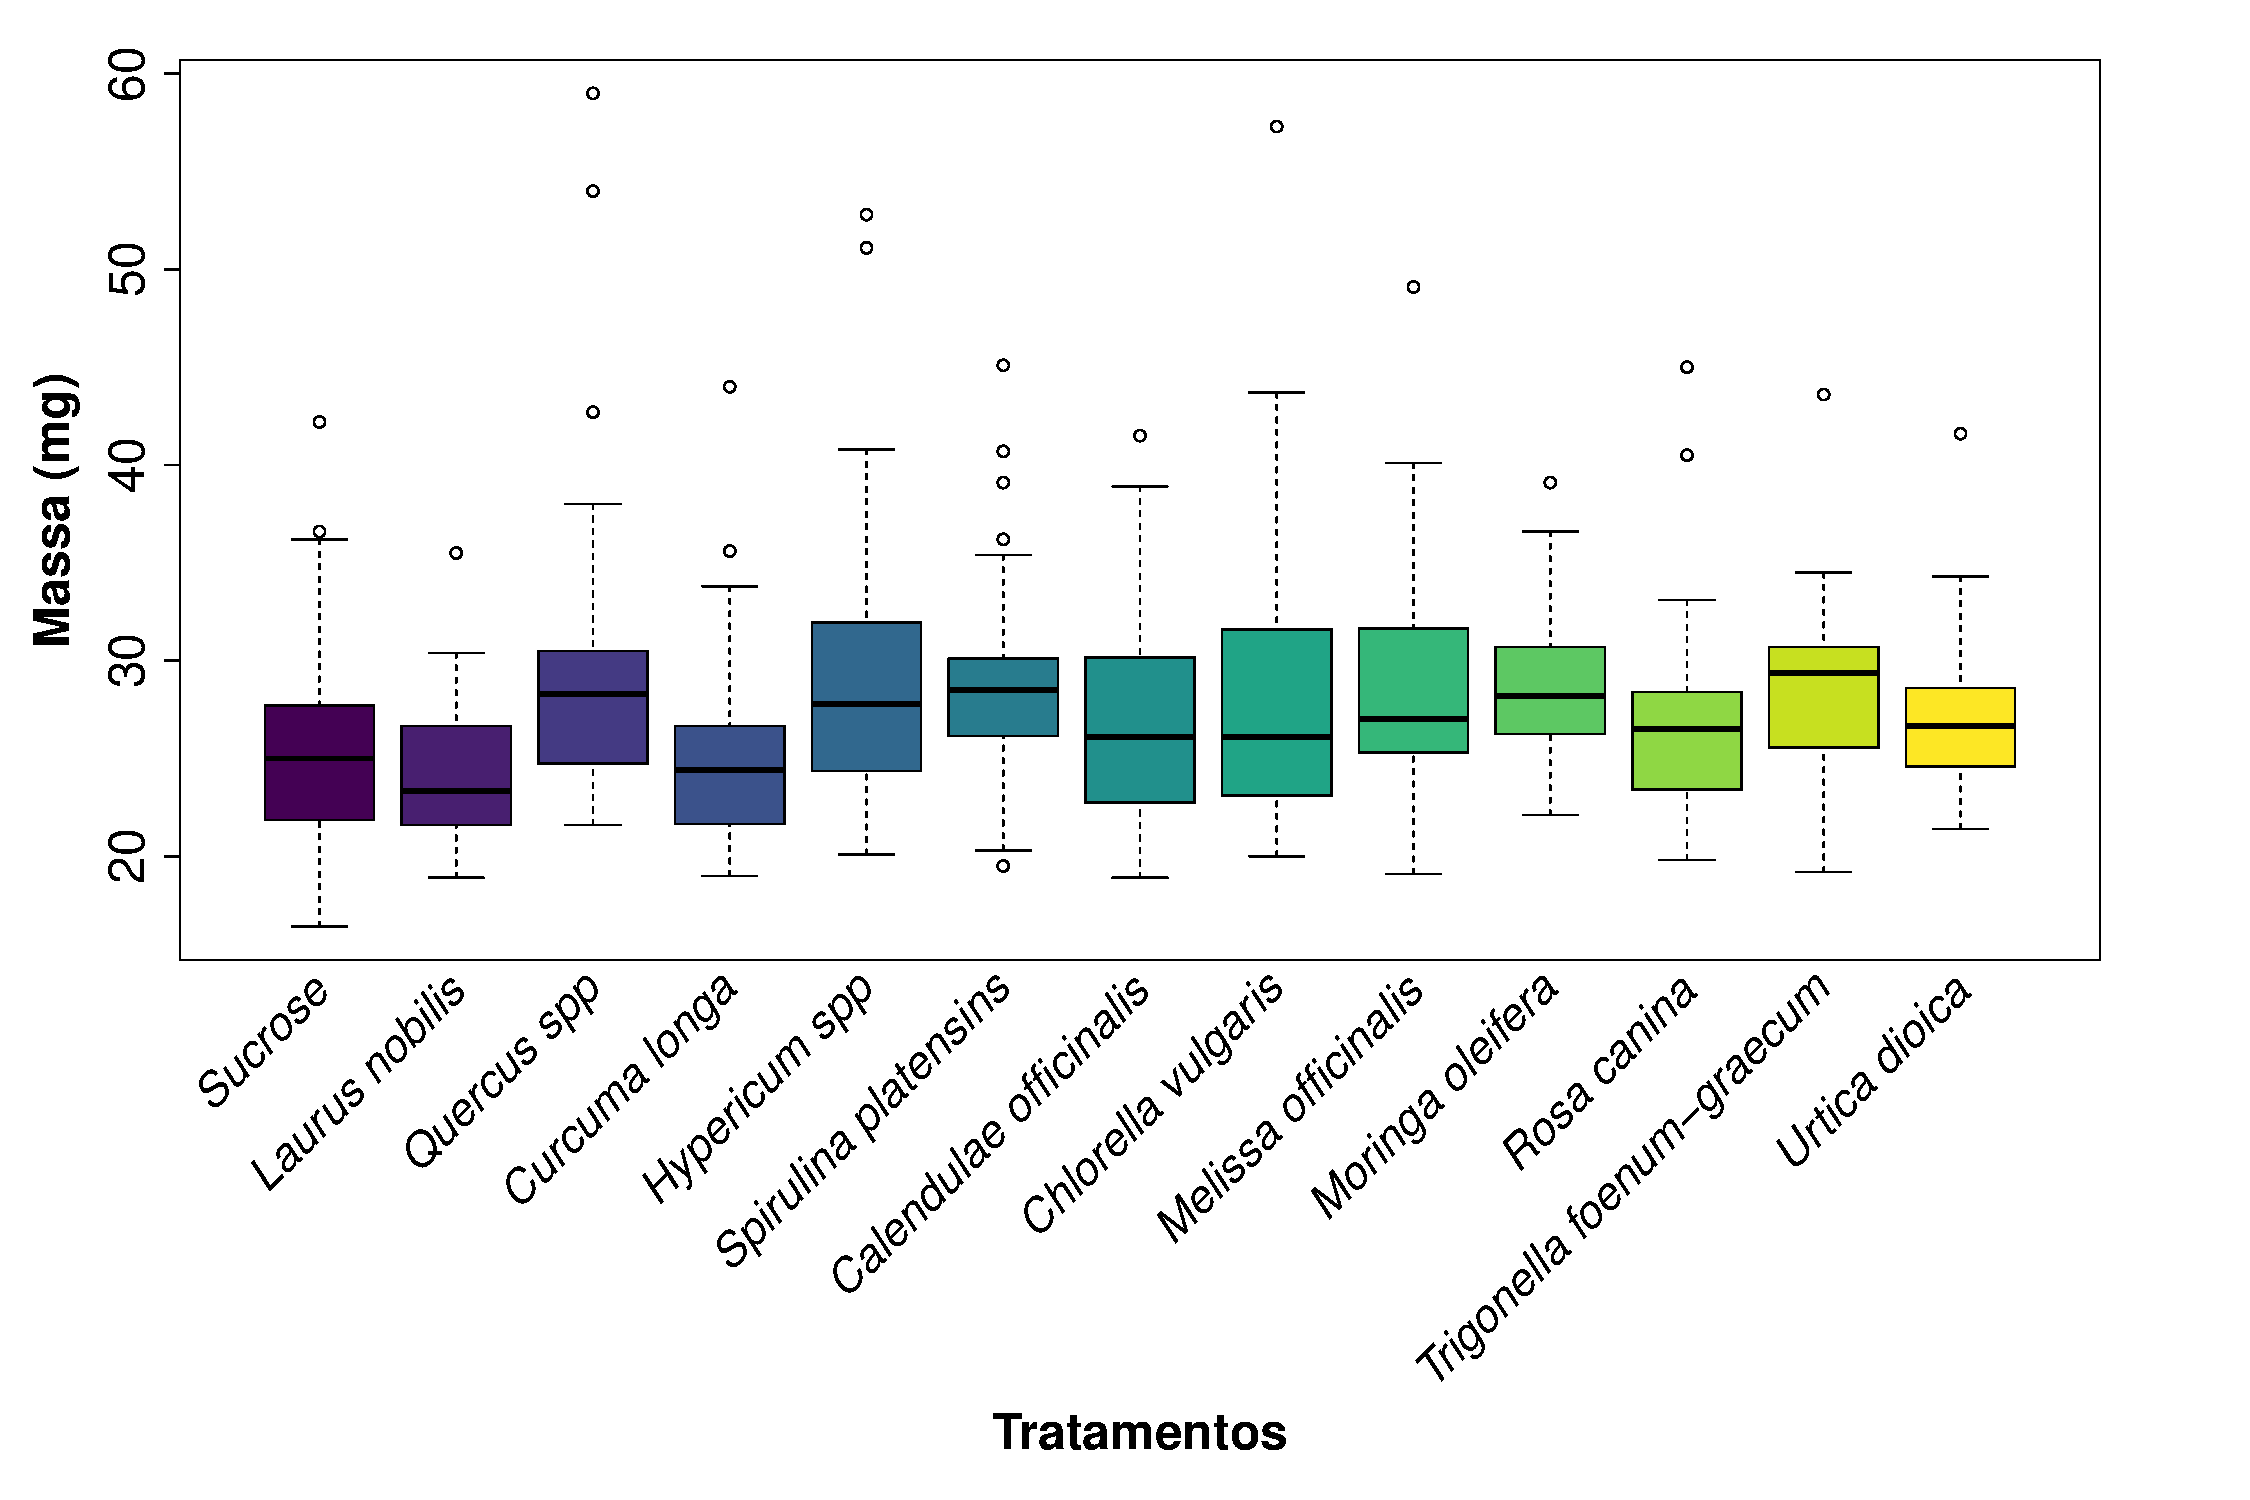
\includegraphics[keepaspectratio]{codigo_abelhas_files/figure-latex/unnamed-chunk-18-1.pdf}}

\begin{Shaded}
\begin{Highlighting}[]
\NormalTok{model }\OtherTok{\textless{}{-}} \FunctionTok{lm}\NormalTok{(df\_weight}\SpecialCharTok{$}\NormalTok{dry\_weight}\SpecialCharTok{\textasciitilde{}}\NormalTok{df\_weight}\SpecialCharTok{$}\NormalTok{day)}
\FunctionTok{summary}\NormalTok{(model)}
\end{Highlighting}
\end{Shaded}

\begin{verbatim}
## 
## Call:
## lm(formula = df_weight$dry_weight ~ df_weight$day)
## 
## Residuals:
##        Min         1Q     Median         3Q        Max 
## -0.0109830 -0.0040330 -0.0008583  0.0022417  0.0310417 
## 
## Coefficients:
##                Estimate Std. Error t value Pr(>|t|)    
## (Intercept)   2.681e-02  8.763e-04  30.593   <2e-16 ***
## df_weight$day 8.218e-05  7.912e-05   1.039    0.299    
## ---
## Signif. codes:  0 '***' 0.001 '**' 0.01 '*' 0.05 '.' 0.1 ' ' 1
## 
## Residual standard error: 0.005933 on 457 degrees of freedom
##   (9 observations deleted due to missingness)
## Multiple R-squared:  0.002355,   Adjusted R-squared:  0.0001723 
## F-statistic: 1.079 on 1 and 457 DF,  p-value: 0.2995
\end{verbatim}

\begin{Shaded}
\begin{Highlighting}[]
\FunctionTok{anova}\NormalTok{(model)}
\end{Highlighting}
\end{Shaded}

\begin{longtable}[]{@{}lrrrrr@{}}
\toprule\noalign{}
& Df & Sum Sq & Mean Sq & F value & Pr(\textgreater F) \\
\midrule\noalign{}
\endhead
\bottomrule\noalign{}
\endlastfoot
df\_weight\$day & 1 & 0.0000380 & 3.80e-05 & 1.078948 & 0.2994823 \\
Residuals & 457 & 0.0160858 & 3.52e-05 & NA & NA \\
\end{longtable}

\subsection{Análise Crítica do Ajuste do Modelo Linear para Peso Seco}

Os autores ajustaram um modelo de regressão linear simples para avaliar
o comportamento do peso seco corporal (\(Y\)) em função do tempo em dias
(\(X\)). A análise do \textit{output} gerado indica que o ajuste do
modelo é extremamente fraco e estatisticamente inadequado para explicar
o fenômeno pelos seguintes motivos:

\begin{enumerate}
    \item \textbf{Ausência de Significância Estatística do Efeito Temporal:}
    O coeficiente angular associado à variável tempo ($\hat{\beta}_1 = 8,218 \times 10^{-5}$) apresenta um erro-padrão de $7,912 \times 10^{-5}$, resultando em um valor da estatística de teste $t = 1,039$. O p-valor correspondente é de $0,299$ ($p > 0,05$). Portanto, não há evidências estatísticas para rejeitar a hipótese nula de que $\beta_1 = 0$, o que indica que o tempo não possui efeito linear significativo sobre o peso seco das abelhas.
    
    \item \textbf{Coeficiente de Determinação Próximo a Zero ($R^2$):}
    O coeficiente de determinação múltiplo ($R^2 = 0,002355$) revela que apenas $0,23\%$ da variabilidade total do peso seco corporal é explicada pela variação dos dias. O $R^2$ ajustado ($0,0001723$) é virtualmente nulo, indicando que o modelo linear estruturado não possui qualquer poder preditivo ou explicativo.
    
    \item \textbf{Insuficiência do Teste $F$ Global:}
    O teste $F$ de significância global da regressão resultou em uma estatística $F = 1,079$ para $1$ e $457$ graus de liberdade, com um p-valor associado de $0,2995$. Isso confirma que o modelo linear proposto não é estatisticamente superior a um modelo ingênuo baseado puramente na média amostral dos pesos ($\bar{Y}$).
\end{enumerate}

\subsection{Teste não paramétrico de
Kruskal-Wallis}\label{teste-nuxe3o-paramuxe9trico-de-kruskal-wallis}

\textbf{Estratégia Estatística e Computacional:} Como os pressupostos de
normalidade dos resíduos foram violados, a estratégia adotada seguiu uma
abordagem não paramétrica, estruturada em três passos:

\begin{enumerate}
    \item \textbf{Cálculo das Diferenças de Mediana:} Determinou-se a mediana de peso seco de cada grupo vegetal e subtraiu-se a mediana do grupo controle ($\Delta\text{Mediana} = \text{Mediana}_{\text{Tratamento}} - \text{Mediana}_{\text{Controle}}$) para quantificar o ganho ou perda de biomassa absoluto.
    \item \textbf{Testes de Hipóteses Individuais:} Utilizou-se o teste de soma de postos de Wilcoxon (Mann-Whitney) para realizar as comparações múltiplas entre os grupos. Computacionalmente, o teste foi executado sem ajustes automáticos globais para permitir o isolamento exclusivo dos 12 contrastes de interesse (cada tratamento \textit{versus} a sacarose pura).
    \item \textbf{Controle de Multiplicidade (FDR):} Aplicou-se a correção de Benjamini-Hochberg (BH) estritamente sobre o vetor dos 12 p-valores gerados contra o controle. Essa estratégia controla a Taxa de Falsas Descobertas, garantindo que o nível de significância global ($\alpha = 0,05$) seja respeitado.
\end{enumerate}

\begin{verbatim}
##                             Treatment Median_difference_mg p_value
## 1             Sucrose: Laurus nobilis                -1.65    0.28
## 2                Sucrose: Quercus spp                 3.30    0.01
## 3              Sucrose: Curcuma longa                -0.60    0.59
## 4              Sucrose: Hypericum spp                 2.80    0.04
## 5       Sucrose: Spirulina platensins                 3.50    0.01
## 6     Sucrose: Calendulae officinalis                 1.10    0.34
## 7         Sucrose: Chlorella vulgaris                 1.10    0.19
## 8        Sucrose: Melissa officinalis                 2.00    0.04
## 9           Sucrose: Moringa oleifera                 3.20    0.01
## 10               Sucrose: Rosa canina                 1.50    0.21
## 11 Sucrose: Trigonella foenum-graecum                 4.35    0.01
## 12             Sucrose: Urtica dioica                 1.65    0.10
\end{verbatim}

\subsection{Crítica Metodológica: Dependência Temporal e Agrupamento}

O artigo original tenta modelar o peso seco corporal (\(dry\_weight\))
inicialmente por meio de uma regressão linear simples baseada no tempo
(\(day\)), agrupando posteriormente os dados dos dias 7 e 14 para
aplicar o teste não paramétrico de Kruskal-Wallis. Contudo, essa
abordagem apresenta uma limitação metodológica importante.

A variável resposta foi coletada em dois momentos distintos no tempo
para as mesmas unidades experimentais (as gaiolas de confinamento ou
\textit{hoarding cages}). Para a aplicação válida tanto da regressão
quanto do teste de Kruskal-Wallis, exige-se o pressuposto fundamental de
que as observações sejam completamente independentes, tanto dentro de
cada grupo quanto entre os grupos estudados.

Ao tratar cada abelha-operária como uma observação isolada, esse
pressuposto é violado duplamente: primeiro, há dependência dentro do
grupo porque abelhas que compartilham a mesma gaiola estão sujeitas ao
mesmo microambiente e comportamento de consumo; segundo, há dependência
entre os tempos (grupos dos dias 7 e 14) porque as medições subsequentes
foram realizadas nas mesmas gaiolas ao longo do tempo. Essa correlação
intraclasse (dependência de agrupamento e temporal) gera uma quebra de
independência dos resíduos (\(\varepsilon\)), infla artificialmente o
tamanho amostral efetivo e distorce os erros-padrão e os p-valores da
análise.

\subsection{Abordagem Estatística Ideal: Modelos Lineares de Efeitos Mistos (LMM)}

Para corrigir a especificação incorreta sem desconsiderar a estrutura
longitudinal dos dados, a estratégia estatística ideal consiste no
ajuste de um \textbf{Modelo Linear de Efeitos Mistos (LMM)}. Esse modelo
decompõe a variabilidade em efeitos fixos e efeitos aleatórios.

Matematicamente, o modelo com \textbf{intercepto aleatório} é expresso
por:

\begin{equation}
Y_{ijk} = \beta_0 + \beta_1 \cdot \text{Treatment}_i + \beta_2 \cdot \text{Day}_j + b_k \cdot I_k + \varepsilon_{ijk}
\end{equation}

Onde:

\begin{itemize}
    \item $Y_{ijk}$ representa o peso seco observado para a abelha no $j$-ésimo dia, sob o $i$-ésimo tratamento, pertencente à $k$-ésima gaiola.
    \item $\beta_0, \beta_1, \beta_2$ são os parâmetros associados aos \textbf{efeitos fixos} do intercepto global, do tratamento e do tempo, respectivamente.
    \item $b_k$ representa o \textbf{efeito aleatório de intercepto} associado à $k$-ésima gaiola, onde $b_k \sim N(0, \sigma^2_b)$. Ele captura a variabilidade sistemática existente entre as diferentes repetições experimentais.
    \item $I_k$ é a \textbf{variável indicadora de agrupamento} (gaiola), que assume valor $I_k = 1$ se a abelha pertence à gaiola $k$, e $I_k = 0$ caso contrário.
    \item $\varepsilon_{ijk}$ é o erro estocástico residual individual, onde $\varepsilon_{ijk} \sim N(0, \sigma^2)$.
\end{itemize}

\section{Sobrevivência}\label{sobrevivuxeancia}

A variável sobrevivência foi obtida por meio do acompanhamento
individual de cada abelha ao longo de todo o experimento. Diariamente,
registrava-se se cada indivíduo permanecia vivo ou se havia ocorrido o
óbito, sendo esse monitoramento realizado até a morte da última abelha.

\textcolor{red}{Como o experimento foi encerrado apenas após a morte de todos os indivíduos, praticamente não houve observações censuradas, uma vez que todas as abelhas apresentaram o evento de interesse (morte) antes do término do estudo.}

O banco de dados de sobrevivência foi composto por uma observação para
cada abelha, totalizando 2028 registros.

As principais variáveis consideradas nessa análise foram:

\begin{itemize}
    \item tratamento;
    \item tempo até a morte (em dias);
    \item status do indivíduo (morreu).
\end{itemize}

\subsubsection{Objetivo da análise}

A análise de sobrevivência teve como objetivo comparar a longevidade das
abelhas submetidas aos diferentes tratamentos, verificando se a
suplementação da solução de sacarose com diferentes pós vegetais
aumentava o tempo de vida das abelhas em relação ao tratamento controle.

\begin{Shaded}
\begin{Highlighting}[]
\FunctionTok{library}\NormalTok{(readxl)}
\FunctionTok{library}\NormalTok{(dplyr)}
\NormalTok{df\_survival }\OtherTok{\textless{}{-}} \FunctionTok{read\_excel}\NormalTok{(}\StringTok{"Plant{-}Powder{-}All{-}Data{-}Final.xlsx"}\NormalTok{, }\AttributeTok{sheet =} \DecValTok{2}\NormalTok{)}
\FunctionTok{head}\NormalTok{(df\_survival,}\DecValTok{8}\NormalTok{)}
\end{Highlighting}
\end{Shaded}

\begin{longtable}[]{@{}rrrlrr@{}}
\toprule\noalign{}
cage & day & individual & treatment & removed & status \\
\midrule\noalign{}
\endhead
\bottomrule\noalign{}
\endlastfoot
2 & 7 & 1 & Sucrose & 3 & 0 \\
2 & 7 & 2 & Sucrose & 3 & 0 \\
2 & 7 & 3 & Sucrose & 3 & 0 \\
2 & 14 & 4 & Sucrose & 3 & 0 \\
2 & 14 & 5 & Sucrose & 3 & 0 \\
2 & 14 & 6 & Sucrose & 3 & 0 \\
2 & 21 & 7 & Sucrose & 1 & 1 \\
2 & 22 & 8 & Sucrose & 1 & 1 \\
\end{longtable}

\begin{Shaded}
\begin{Highlighting}[]
\FunctionTok{kable}\NormalTok{(}\FunctionTok{slice}\NormalTok{(df\_survival, }\DecValTok{19}\SpecialCharTok{:}\DecValTok{27}\NormalTok{), }\AttributeTok{digits =} \DecValTok{3}\NormalTok{)}
\end{Highlighting}
\end{Shaded}

\begin{longtable}[]{@{}rrrlrr@{}}
\toprule\noalign{}
cage & day & individual & treatment & removed & status \\
\midrule\noalign{}
\endhead
\bottomrule\noalign{}
\endlastfoot
2 & 38 & 19 & Sucrose & 1 & 1 \\
2 & 40 & 20 & Sucrose & 1 & 1 \\
2 & 44 & 21 & Sucrose & 1 & 1 \\
2 & 45 & 22 & Sucrose & 1 & 1 \\
2 & 46 & 23 & Sucrose & 1 & 1 \\
2 & 48 & 24 & Sucrose & 1 & 1 \\
3 & 7 & 1 & Sucrose & 3 & 0 \\
3 & 7 & 2 & Sucrose & 3 & 0 \\
3 & 7 & 3 & Sucrose & 3 & 0 \\
\end{longtable}

\begin{Shaded}
\begin{Highlighting}[]
\NormalTok{df\_survival}\SpecialCharTok{$}\NormalTok{treatment }\OtherTok{\textless{}{-}} \FunctionTok{factor}\NormalTok{(df\_survival}\SpecialCharTok{$}\NormalTok{treatment,}
                                \AttributeTok{levels =} \FunctionTok{c}\NormalTok{(}\StringTok{"Sucrose"}\NormalTok{,}\StringTok{"Laurus nobilis"}\NormalTok{,}\StringTok{"Quercus spp"}\NormalTok{, }\StringTok{"Curcuma longa"}\NormalTok{,}
                                \StringTok{"Hypericum spp"}\NormalTok{,}\StringTok{"Spirulina platensins"}\NormalTok{, }\StringTok{"Calendulae officinalis"}\NormalTok{,}
                                \StringTok{"Chlorella vulgaris"}\NormalTok{, }\StringTok{"Melissa officinalis"}\NormalTok{,}\StringTok{"Moringa oleifera"}\NormalTok{,}
                                \StringTok{"Rosa canina"}\NormalTok{,}\StringTok{"Trigonella foenum{-}graecum"}\NormalTok{, }\StringTok{"Urtica dioica"}\NormalTok{))}

\NormalTok{tabela\_4\_direta }\OtherTok{\textless{}{-}}\NormalTok{ df\_survival }\SpecialCharTok{\%\textgreater{}\%}
  \FunctionTok{group\_by}\NormalTok{(treatment) }\SpecialCharTok{\%\textgreater{}\%}
  \FunctionTok{summarise}\NormalTok{(}\AttributeTok{Minimum =} \FunctionTok{min}\NormalTok{(day, }\AttributeTok{na.rm =} \ConstantTok{TRUE}\NormalTok{),}
            \StringTok{\textasciigrave{}}\AttributeTok{1st quartile}\StringTok{\textasciigrave{}} \OtherTok{=} \FunctionTok{quantile}\NormalTok{(day, }\FloatTok{0.25}\NormalTok{, }\AttributeTok{na.rm =} \ConstantTok{TRUE}\NormalTok{),}
            \AttributeTok{Median =} \FunctionTok{median}\NormalTok{(day, }\AttributeTok{na.rm =} \ConstantTok{TRUE}\NormalTok{),}
            \StringTok{\textasciigrave{}}\AttributeTok{3rd quartile}\StringTok{\textasciigrave{}} \OtherTok{=} \FunctionTok{quantile}\NormalTok{(day, }\FloatTok{0.75}\NormalTok{, }\AttributeTok{na.rm =} \ConstantTok{TRUE}\NormalTok{),}
            \AttributeTok{Maximum =} \FunctionTok{max}\NormalTok{(day, }\AttributeTok{na.rm =} \ConstantTok{TRUE}\NormalTok{)) }\SpecialCharTok{\%\textgreater{}\%}
  \FunctionTok{ungroup}\NormalTok{() }\SpecialCharTok{\%\textgreater{}\%}
\NormalTok{  dplyr}\SpecialCharTok{::}\FunctionTok{rename}\NormalTok{(}\AttributeTok{Treatment =}\NormalTok{ treatment)}
\FunctionTok{print}\NormalTok{(tabela\_4\_direta)}
\end{Highlighting}
\end{Shaded}

\begin{verbatim}
## # A tibble: 13 x 6
##    Treatment                Minimum `1st quartile` Median `3rd quartile` Maximum
##    <fct>                      <dbl>          <dbl>  <dbl>          <dbl>   <dbl>
##  1 Sucrose                        7           16       29           34        61
##  2 Laurus nobilis                 1           14       31           40        61
##  3 Quercus spp                    3           14       33           42        69
##  4 Curcuma longa                  2           15.5     31           39        68
##  5 Hypericum spp                  2           14       29           41        66
##  6 Spirulina platensins           3           14       28           39        59
##  7 Calendulae officinalis         4           14       28           38        56
##  8 Chlorella vulgaris             1           14       33           41        66
##  9 Melissa officinalis            4           14       29           43.8      66
## 10 Rosa canina                    6           15       32           39        58
## 11 Trigonella foenum-graec~       4           16.5     33           41        57
## 12 Urtica dioica                  3           14       35           46        63
## 13 <NA>                           3           14       27           38        53
\end{verbatim}

\begin{Shaded}
\begin{Highlighting}[]
\FunctionTok{qf}\NormalTok{(}\FloatTok{0.95}\NormalTok{,}\DecValTok{4}\NormalTok{,}\DecValTok{5}\NormalTok{)}
\end{Highlighting}
\end{Shaded}

\begin{verbatim}
## [1] 5.192168
\end{verbatim}

\begin{Shaded}
\begin{Highlighting}[]
\FunctionTok{qt}\NormalTok{(}\FloatTok{0.975}\NormalTok{,}\DecValTok{9}\NormalTok{)}
\end{Highlighting}
\end{Shaded}

\begin{verbatim}
## [1] 2.262157
\end{verbatim}

\begin{Shaded}
\begin{Highlighting}[]
\FunctionTok{library}\NormalTok{(survival)}
\FunctionTok{library}\NormalTok{(survminer)}

\FunctionTok{par}\NormalTok{(}\AttributeTok{mar=}\FunctionTok{c}\NormalTok{(}\DecValTok{7}\NormalTok{,}\DecValTok{8}\NormalTok{,}\DecValTok{2}\NormalTok{,}\DecValTok{6}\NormalTok{)) }\CommentTok{\# set margins}
\FunctionTok{par}\NormalTok{(}\AttributeTok{mfrow =} \FunctionTok{c}\NormalTok{(}\DecValTok{1}\NormalTok{,}\DecValTok{1}\NormalTok{)) }\CommentTok{\# will do 2 plots next to eachother}
\NormalTok{fit}\OtherTok{\textless{}{-}}\FunctionTok{survfit}\NormalTok{(}\FunctionTok{Surv}\NormalTok{(df\_survival}\SpecialCharTok{$}\NormalTok{day, df\_survival}\SpecialCharTok{$}\NormalTok{status)}\SpecialCharTok{\textasciitilde{}}\NormalTok{df\_survival}\SpecialCharTok{$}\NormalTok{treatment)}
\NormalTok{lev}\OtherTok{\textless{}{-}}\FunctionTok{length}\NormalTok{(}\FunctionTok{levels}\NormalTok{(df\_survival}\SpecialCharTok{$}\NormalTok{treatment))}

\NormalTok{ggcolors }\OtherTok{\textless{}{-}} \FunctionTok{c}\NormalTok{(}\StringTok{"\#440154FF"}\NormalTok{,}\StringTok{"\#481F70FF"}\NormalTok{,}\StringTok{"\#443A83FF"}\NormalTok{,}\StringTok{"\#3B528BFF"}\NormalTok{,}\StringTok{"\#31688EFF"}\NormalTok{,}
              \StringTok{"\#287C8EFF"}\NormalTok{,}\StringTok{"\#21908CFF"}\NormalTok{,}\StringTok{"\#20A486FF"}\NormalTok{,}\StringTok{"\#35B779FF"}\NormalTok{,}\StringTok{"\#5DC863FF"}\NormalTok{,}
              \StringTok{"\#8FD744FF"}\NormalTok{,}\StringTok{"\#C7E020FF"}\NormalTok{,}\StringTok{"\#FDE725FF"}\NormalTok{)}

\FunctionTok{plot}\NormalTok{(fit, }\AttributeTok{col=}\NormalTok{ggcolors, }\AttributeTok{yaxt=}\StringTok{"n"}\NormalTok{,}\AttributeTok{yaxs=}\StringTok{"r"}\NormalTok{,}\AttributeTok{lwd=}\DecValTok{4}\NormalTok{,}\AttributeTok{pch=}\DecValTok{10}\NormalTok{,}\AttributeTok{cex=}\DecValTok{3}\NormalTok{,}\AttributeTok{mark.time=}\NormalTok{T, }\AttributeTok{cex.lab =} \DecValTok{2}\NormalTok{,}
     \AttributeTok{xlab =} \StringTok{"Tempo (dias)"}\NormalTok{, }\AttributeTok{ylab =} \StringTok{"Probabilidade de sobrevivência (\%)"}\NormalTok{,}
     \AttributeTok{cex.axis=}\DecValTok{2}\NormalTok{, }\AttributeTok{font.lab=}\DecValTok{2}\NormalTok{,}\AttributeTok{frame.plot=}\NormalTok{T); }
\FunctionTok{axis}\NormalTok{(}\AttributeTok{side=}\DecValTok{2}\NormalTok{, }\AttributeTok{at=}\FunctionTok{pretty}\NormalTok{(fit}\SpecialCharTok{$}\NormalTok{surv), }\AttributeTok{cex.axis=}\DecValTok{2}\NormalTok{,}
     \AttributeTok{lab=}\FunctionTok{paste0}\NormalTok{(}\FunctionTok{pretty}\NormalTok{(fit}\SpecialCharTok{$}\NormalTok{surv) }\SpecialCharTok{*} \DecValTok{100}\NormalTok{), }\AttributeTok{las=}\ConstantTok{TRUE}\NormalTok{)}
\FunctionTok{legend}\NormalTok{(}\FloatTok{44.5}\NormalTok{, }\DecValTok{1}\NormalTok{,  }\FunctionTok{levels}\NormalTok{(df\_survival}\SpecialCharTok{$}\NormalTok{treatment), }\AttributeTok{col=}\NormalTok{ggcolors, }\AttributeTok{lwd=}\DecValTok{4}\NormalTok{,}\AttributeTok{cex =} \FloatTok{1.5}\NormalTok{)}
\end{Highlighting}
\end{Shaded}

\pandocbounded{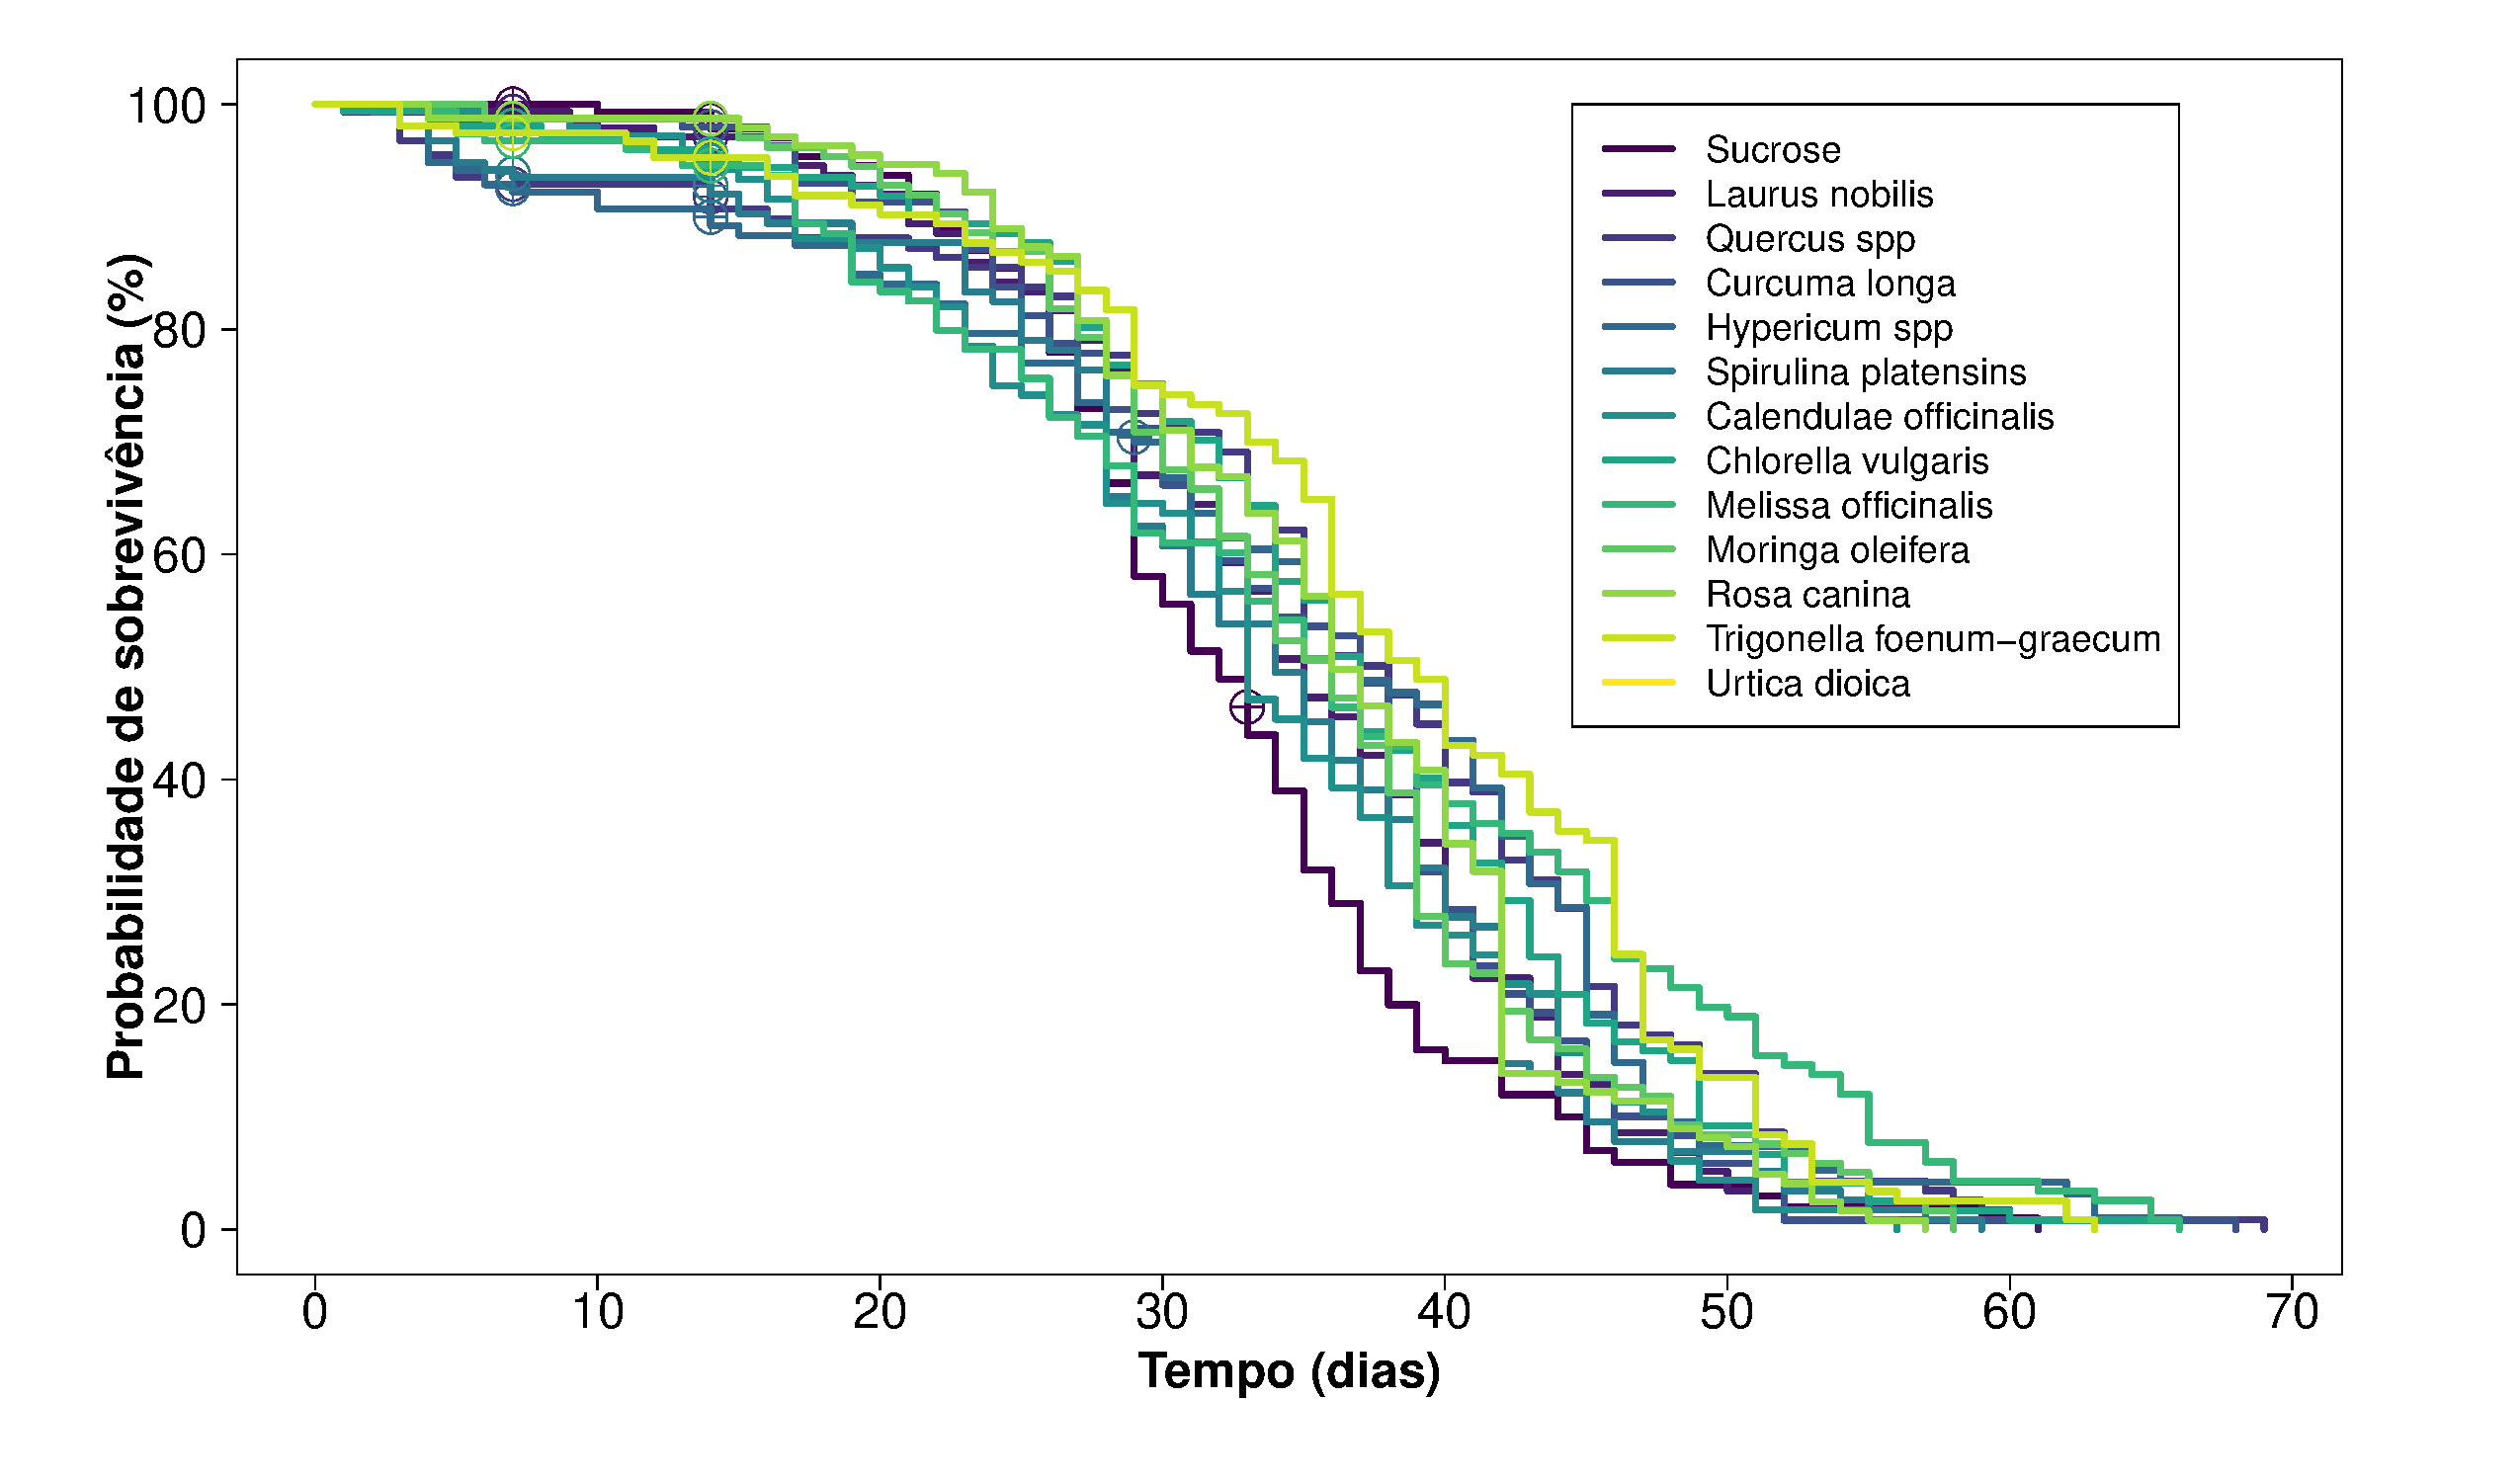
\includegraphics[keepaspectratio]{codigo_abelhas_files/figure-latex/unnamed-chunk-22-1.pdf}}

\end{document}
